\subsubsection{Evaluation Strategy}

\paragraph{Hovering}

We implemented a 1D control mission: regulating the drone's vertical position ($y$) within a target band $[H - R, H + R]$, where $H$ is the `targetHeight` and $R$ is the `acceptableRadius`.

To monitor progress, we implemented a color-coded feedback system, \cref{fig:train}: Yellow: Below target; Orange: Above target; Blue: Stable hovering.

\begin{figure}[H]
    \caption{training process}\label{fig:train}
    \centering
    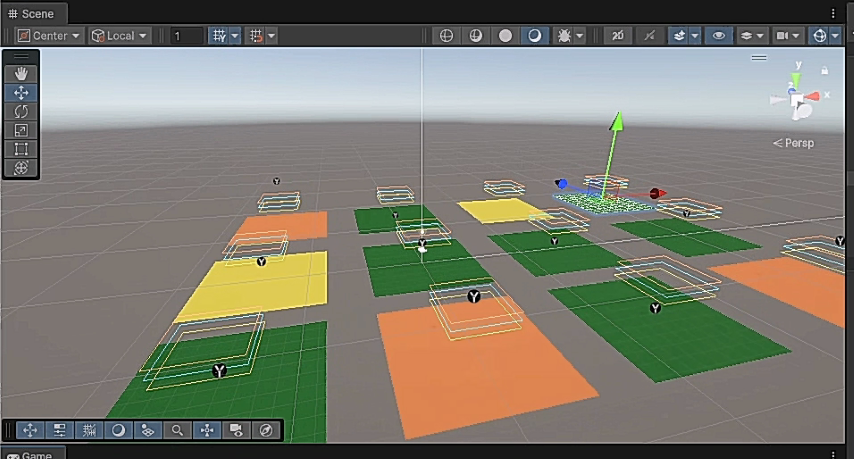
\includegraphics[width=0.8\linewidth]{img/train.png}
\end{figure}



\paragraph{Path Following}
A simple path following task can be used to test if the Human-AI Collaboration Agent meets our expectation.

To implement path following, two other components are included, PathFollower, cut the path into different targets for PidDroneEmulator to calculate errors and PathGenerator to build the path.

To move between points, the PathGenerator generates a path using two Cubic Bézier curves. Given four control points $P_0, P_1, P_2, P_3$, home to waypoint and back, the position $B(t)$ for $t \in [0,1]$ is defined as \cref{eq:bezier}.

\begin{equation}\label{eq:bezier}
    B(t) = {(1-t)}^3 P_0 + 3{(1-t)}^2 t P_1 + 3(1-t) t^2 P_2 + t^3 P_3
\end{equation}

The path is constructed relative to the Home and Target vectors, the drone will fly from Home and fly back, the path as shown in \cref{fig:path_design}. Path from Home to Waypoint using a right-hand offset for control points; Path from Waypoint back to Home using a left-hand offset.

\begin{figure}[H]
    \caption{Path Design}\label{fig:path_design}
    \centering
    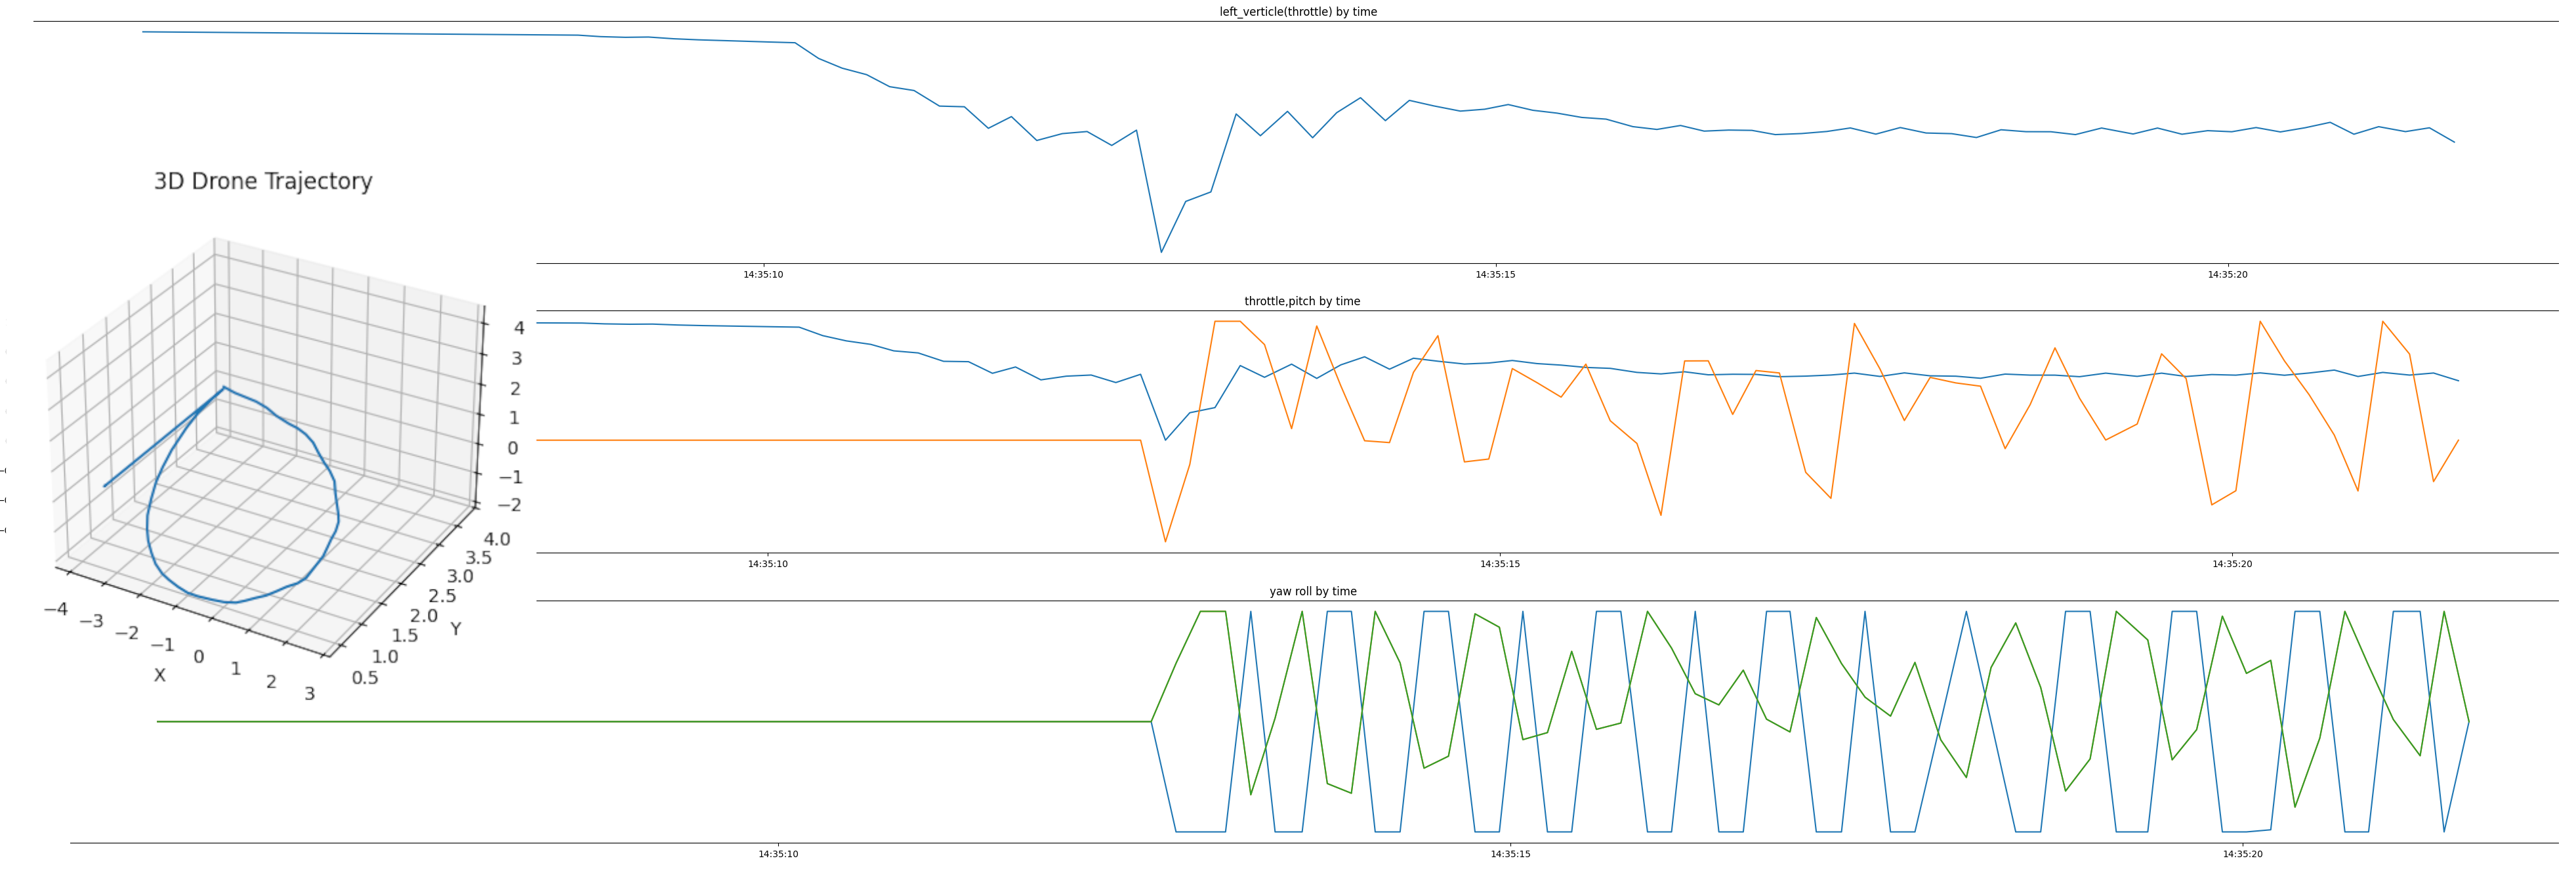
\includegraphics[width=0.8\linewidth]{img/path.png}
\end{figure}

By calculating these normalized joystick rates, For both the path following task and the hovering task, the system can visualize the AI's calculation on the HUD. So that the evaluation method can be delivered in a flat panel display, no need of XR devices.
